%!TEX root = ../thesis.tex
%*******************************************************************************
%*********************************** First Chapter *****************************
%*******************************************************************************

\chapter{Introduction}  %Title of the First Chapter

\ifpdf
    \graphicspath{{Chapter1/Figs/Raster/}{Chapter1/Figs/PDF/}{Chapter1/Figs/}}
\else
    \graphicspath{{Chapter1/Figs/Vector/}{Chapter1/Figs/}}
\fi

Somatic mutations can occur in cells at all stages of life and in all tissues. Somatic mutational processes in asexually reproducing cells and in the germline of sexually producing species generates genetic diversity and ultimately, phenotypic diversity. Natural and sexual selection act upon individuals with different phenotypes to drive adaption and selection. 

The completion of the Human Genome Project (HGP) \cite{Lander2001-du} and the advent of next-generation sequencing platform \cite{Bentley2008-kl} have made it possible to detect and analyse somatic mutations of thousands of tumours \cite{Weinstein2013-ko, ICGCTCGA_Pan-Cancer_Analysis_of_Whole_Genomes_Consortium2020-ts}. In stark contrast, the inability to detect somatic mutations in normal tissues at scale and the high cost associated with constructing high-quality reference genomes have hindered the characterisation of somatic mutational processes across the Tree of Life. The ability to produce long and accurate reads through circular consensus sequencing (CCS) from Pacific Biosciences (PacBio) \cite{Wenger2019-pw} has sparked interest for \textit{de novo} assembly of genomes across the Tree of Life \cite{Darwin_Tree_of_Life_Project_Consortium2022-ma}. Here, I describe a new method that uses CCS reads to enable the detection of somatic mutations present as a single copy from bulk normal tissue. I also discuss application of this method to discovering new somatic mutational processes across the Tree of Life. 

\section{The somatic mutation landscape of \textit{H. sapiens}}

To date, the study of somatic mutagenesis has primarily focused on \textit{H. sapiens} and somatic mutations present in clones of cells as part of ongoing efforts to describe the landscape of driver mutations in tumors. The contribution of somatic mutations to oncogenesis was first implicated as early as 1890 by Friedrich von Hansemann, who observed aberrant chromosomal alterations in cancer cells under the microscope \cite{hansemann_1890}.

The continued decline in sequencing costs and the concurrent development of somatic mutation detection algorithms have enabled the characterisation of somatic mutations in thousands of tumour samples \cite{Weinstein2013-ko, ICGCTCGA_Pan-Cancer_Analysis_of_Whole_Genomes_Consortium2020-ts}. Although most somatic mutations are benign (passenger mutations), some somatic mutations can confer a proliferative advantage to a cell and are classified as driver mutations. The detection of these driver mutations and their subsequent association with the hallmarks of cancer \cite{Hanahan2000-dp, Hanahan2011-zr} has been one of the primary motivations for cataloguing somatic mutations in cancer genomes. In more recent times, somatic mutation detection in normal cells has become increasingly important to lineage trace embryonic development \cite{Behjati2014-gb} and to understand the transformation of normal cells to neoplastic cells \cite{Martincorena2015-io}. 

\subsection{Somatic mutation detection in tumours}
\label{sec:somatic_mutation_detection_in_tumours}

Cancer is often described as the disease of the genome. The acquisition of driver mutations through a single event such as chromothripsis \cite{Stephens2011-gj} or gradual accumulation of somatic mutations \cite{Doll1954-of, Knudson1971-fg} is one of the primary contributors to tumorigenesis. Hence, somatic mutation detection is often the first step towards characterising the cancer genome. 

Unlike germline mutations, where approximately 50\% and 100\% of reads support the germline mutation, somatic mutations in tumour tissues can have a variant allele fraction (VAF) that ranges from 0-100\% depending on their purity, cell clonality and copy number changes. Given that tumour samples frequently consist of a mixture of normal and cancer cells, accurately measuring the variant allele fraction (VAF) of somatic mutations can pose a challenge. Moreover, the copy number of the chromosome can fluctuate substantially in the cancer genome as a result of chromothripsis \cite{Stephens2011-gj}, aberrant chromosomal alternations \cite{Albertson2003-lr, Frohling2008-uc} or loss of heterozygosity (LOH) \cite{Lasko1991-wq}. Furthermore, library errors that damage the template molecule before sequencing, as well as genomic DNA (gDNA) contamination, are other critical factors that must be considered in somatic mutation detection.

A matched tumour-normal sequencing is often performed to distinguish germline mutations from somatic mutations and to detect somatic mutations present in a clone of cells. The presence of a matched normal also enables the calculation of tumour purity, the proportion of cancer cells in a tumour sample, which is another critical component that determines somatic mutation detection sensitivity. Germline mutations detected in the matched normal serves as a reference panel to determine whether the mutation detected in the tumour sample is a germline mutation or a somatic mutation. In cases where a tumor sample has low sequence coverage or low tumor purity, there is a possibility of misclassifying heterozygous germline mutations as somatic mutations \cite{Cibulskis2013-gw}.

Each somatic mutation detection algorithm employs a unique strategy to calculate the normal contamination in tumour \cite{Cibulskis2011-tp}, tumour contamination in normal \cite{Taylor-Weiner2018-af} and to differentiate between somatic and germline mutations. For instance, VarScan2 uses a hard filter \cite{Koboldt2012-wd}, MuTect uses a likelihood ratio \cite{Cibulskis2013-gw} and Strelka2 uses a mixture model \cite{Kim2018-qi} based on the number of reads supporting the mutation in the normal and tumour samples to classify each somatic mutation candidate. Since each somatic mutation detection algorithm exhibits varying sensitivity and specificity, as well as different strengths and weaknesses, a consensus somatic mutation call from different somatic mutation algorithms is often used for downstream sequence analysis \cite{Bailey2020-ou}.

During library preparation, DNA damage is introduced to the template molecule, and a set of DNA damage repair enzymes is used to repair it. If DNA damage remains unrepaired or is incorrectly repaired, the template DNA molecule is permanently altered before sequencing. During the sequencing process, base quality (BQ) scores are assigned to individual bases to reflect the uncertainty of each base call. Somatic mutation detection algorithms rely on sequence coverage and BQ scores to calculate the genotype quality (GQ) score of a germline mutation \cite{McKenna2010-br, Li2011-ag} and the confidence with which the somatic mutation is called \cite{Cibulskis2013-gw}. 

Since sequencing instruments cannot determine whether a base in the template molecule is derived from a somatic mutation or a library error, the BQ score does not necessarily indicate the probability that a non-reference base in a read is the result of a mutation. Consequently, low-frequency library errors are often misclassified as somatic mutations, requiring specialized filters to minimize the number of false positive mutations \cite{Costello2013-cz, Chen2017-ba}.

PCR amplification, DNA oxidation and DNA crosslinking (in formalin-fixed tissues) are commonly recognised sources of library errors \cite{Chen2017-ba}. The identification of oxidative DNA damage during sonication-based DNA fragmentation, and the characterisation of read features that facilitate the differentiation between artefactual mutations and somatic mutations, serves as an illustrative example \cite{Costello2013-cz}. Acoustic shearing of DNA oxidizes guanine to 8-oxoguanine (8-oxoG), and the preferential pairing of 8-oxoG with adenine \cite{Shibutani1991-tw} is responsible for the generation of CCG>CAG/CGG>CTG transversions during PCR amplification \cite{Costello2013-cz}. The addition of DNA glycosylases during library preparation can mitigate the effect of DNA oxidation. Furthermore, the sequence context and orientation bias of the mutation can also be assessed to determine the extent of oxidative DNA damage in the library \cite{Costello2013-cz}.


The repeat content of the reference genome is another important factor for somatic mutation detection, often overlooked. Repetitive sequences account for approximately 50\% of the human genome \cite{Lander2001-du}. When the repeat length exceeds the read length, read aligners are unable to determine the precise location of the read within the reference genome, as it could have originated from any of the copies of the repetitive sequence in the genome \cite{Li2008-dt}. Therefore, accurate read placement requires repetitive sequences to be flanked with unique sequences that are not present elsewhere in the reference genome. Alignment errors in low sequence complexity regions are another common source of false positive mutations \cite{Li2014-ra}. As a result, both germline and somatic mutation detection algorithms discard mutations when the total number of mutations in adjacent to the called mutation, within a defined window, exceeds a predefined threshold \cite{Cibulskis2013-gw, DePristo2011-vf}. Consequently, the reference genome is divided into callable and non-callable regions based on the mappability of Illumina short reads, and variant calling is often restricted to the callable regions of the genome \cite{1000_Genomes_Project_Consortium2012-rj}. Hence, clinically relevant genes located in non-callable regions are often excluded from analysis \cite{Wagner2022-ph}.

The completeness of the reference genome is another crucial factor to consider in somatic mutation detection. Even the human reference genome remains incomplete, with missing sequences, unplaced and unlocalized scaffolds, and misassemblies such as erroneous sequence collapse and expansion \cite{Schneider2017-yo}. However, the telomere-to-telomere CHM13 (T2T-CHM13) genome, which is constructed using a combination of sequencing and mapping technologies, currently represents the most accurate and complete human genome available. In comparison to the human reference genome, the T2T-CHM13 genome provides fully resolved sequences for the short arms of acrocentric chromosomes and the centromeres of all chromosomes, except for chromosome Y \cite{Nurk2022-dv}. As expected, the T2T-CHM13 genome significantly improves the accuracy and precision of both read alignment and variant calling \cite{Aganezov2022-dv}.

To account for errors that cannot be eliminated through an analytical approach, a panel of normal (PoN) VCF file is generated from a set of normal samples using the same parameters as those applied in somatic mutation detection. Afterwards, somatic mutation detections found in the PoN VCF are filtered out \cite{Cibulskis2013-gw}.

\subsection{Somatic mutation detection in normal tissue}
\label{sec:somatic_mutation_detection_in_normal_tissue}

An individual begins to accumulate somatic mutations upon fertilisation and the gradual accumulation of driver mutations is one of the principal drivers of tumorigenesis \cite{Stratton2009-of}. The determination of the sequence of events that leads to the transformation of a normal cell into a neoplastic cell requires studying the driver mutation landscape in normal tissue across different ages and individuals with a genetic predisposition to cancer \cite{Martincorena2015-io}. In addition, the ability to detect somatic mutations in normal cells is critical for the earlier detection of cancer and the monitoring of cancer relapse \cite{Newman2014-qq, Newman2016-cy}.

Somatic mutation detection in normal tissue presents a unique set of challenges as somatic mutations are typically present as single copies in a DNA extract from bulk normal tissue, except for mosaic mutations that arise during embryonic development. In tumour samples, somatic mutation detection is feasible if a somatic mutation is present in a clone of cells above the 0.1-1\% Illumina sequencing error rate \cite{Cibulskis2013-gw}. A newly acquired somatic mutation or a somatic mutation with a variant allele fraction (VAF) below the Illumina sequencing error rate cannot be distinguished from background noise. Therefore, the detection of somatic mutations in normal tissue requires either an increase in the copy number of the mutant DNA above the limit of detection threshold or an improvement in the base accuracy of the Illumina reads through upstream changes in the library preparation protocol.

\subsubsection{Single-cell resolution somatic mutation detection}

Both single-cell whole-genome amplification \cite{Lodato2018-hh} and single-cell clone expansion and sequencing \cite{Lee-Six2018-qe, MSpencer_Chapman2021-cq} aims to increase the copy number of the mutant DNA prior to library preparation and sequencing. On the other hand, laser-capture microdissection (LCM) and sequencing leverage spatial partitioning of tissues through histological staining to isolate and sequence a clonal unit of cells, such as the colonic crypt \cite{Ellis2021-it}. Single-cell clone expansion and LCM sequencing are recognised as the gold-standard methods for somatic mutation detection in single cells or clonal tissues, respectively. In contrast, single-cell whole-genome amplification and sequencing has several disadvantages. For instance, allele dropout occurs during PCR amplifciation when one of the two alleles at heterozygous locus is not amplified, leading to a false homozygous mutation call. To date, single-cell clone expansion and LCM sequencing have been successfully used to determine the somatic mutation rate, the somatic mutational processes, and the clonal structure across a range across a range of normal tissues, including adrenal gland, blood, bladder, bronchus, cardiac muscle, colon, endometrium, oesophagus, pancreas, placenta, prostate, skin, smooth muscle, testis, thyroid, ureter, visceral fat \cite{Lee-Six2018-qe, MSpencer_Chapman2021-cq, Martincorena2015-gu, Ju2017-vw, Martincorena2018-av, Brunner2019-xg, Lee-Six2019-vt, Yoshida2020-yr, Olafsson2020-vi, Moore2020-pi, Lawson2020-em, Coorens2021-ct, Robinson2021-te, Grossmann2021-gd, Moore2021-dl, Park2021-fx, Ng2021-jd, Mitchell2022-ry}. 

\subsubsection{Single-molecule resolution somatic mutation detection}

Unfortunately, single-cell clone expansion and LCM sequencing are arduous processes that are difficult to scale up for routine use in clinical settings. In contrast, liquid biopsies utilize duplex sequencing methods to detect driver mutations from circulating tumor DNA (ctDNA) in the plasma, enabling earlier detection of cancers and monitoring of tumor evolution \cite{Newman2016-cy}. Duplex sequencing methods generate multiple copies of the same template molecule and construct a highly accurate consensus sequence, leveraging the redundancies between the copies of the same template molecule and the complementary base pairing between the forward and reverse strands of a double-stranded DNA molecule \cite{Schmitt2012-yr, Hoang2016-jx, Abascal2021-pk}. The recently developed nanorate sequencing protocol enables single-molecule resolution somatic mutation detection \cite{Abascal2021-pk}. 

\subsection{Somatic mutations as biological barcodes}

The fusion of the egg and sperm creates a zygote, whose genome possesses a unique combination of maternal and paternal alleles. The genome of the zygote orchestrates the programmed embryonic development from a single cell to a multicellular organism. Somatic mutations begin to accumulate with the first cell division of an embryo, and cells with the same somatic mutation are assumed to share the same stem cell lineage. Hence, somatic mutations have been used as biological barcodes to facilitate lineage tracing of cells and gain insight into embryonic development and the cellular origin of tissues \cite{Behjati2014-gb}.

The number of somatic mutations in a cell is dependent on the age and somatic mutation rate of the sample. Naturally, paediatric cancers in children exhibit a lower mutation burden compared to adult tumours \cite{Grobner2018-ve}. As a result, the hypothesis that tumours arise from the gradual accumulation of somatic mutations does not apply to paediatric cancers. As an alternative hypothesis, abnormal embryonic development has been proposed to explain paediatric cancers \cite{Marshall2014-ec}. In the former hypothesis, paediatric cancer will have unique set of somatic mutations, while in the latter hypothesis, paediatric cancer will share mosaic mutations and premalignant clones with the neighbouring normal tissue (mosaic mutations are somatic mutations that occur during the first few cell divisions of embryonic development and are shared across multiple tissues). The study of shared somatic mutations in bilateral and unilateral Wilms tumour and adjacent normal kidney tissues supports the latter hypothesis that paediatric cancer arises from aberrant foetal development \cite{Coorens2019-zf}. A similar analysis in bilateral adrenal neuroblastoma also revealed that the left and right adrenal gland tumours do not arise from a single premalignant clone, but rather two independent premalignant clones separated before the first few cell divisions of a zygote \cite{Coorens2020-ut}. Intriguingly, these studies also show that the left-right axis of the kidneys and adrenal glands are established during the early cell divisions of a zygote. 

\subsection{Somatic mutational processes}
\label{sec:mutational_signature_analysis}

Somatic mutational process is a continuous process throughout life, and multiple somatic mutational processes simultaneously act on the cell’s genome at any given time. Mutational signature analysis is performed to determine the somatic mutational processes that have acted upon the genome and measure the contribution of each somatic mutational process to the mutational burden of the sample. Mutational signature analysis can either \textit{de novo} extract new mutational signatures from a catalogue of somatic mutations from multiple samples or use a set of reference mutational signatures to calculate the attribution of each mutational signature to the mutation burden of the sample. A mutational signature is defined as a group of probabilities that represent the likelihood of a somatic mutational process to generating a mutation at specific sequence contexts \cite{Alexandrov2013-fq}.

During mutational signature analysis, somatic mutations are classified according to the event, the size of the event and the sequence context. For example, single base substitutions (SBS) are often classified using the SBS96 classification system. In the pyrimidine sequence context, there are 6 types of substitutions (C>A, C>G, C>T, T>A, T>C and T>G) and 16 possible trinucleotide sequence contexts derived from the 4 bases upstream and downstream of the substitution. This combination of substitutions and trinucleotide sequence contexts forms the basis of the canonical SBS96 classification system. The SBS96 classification systeem can be further expanded to the SBS192 or the SBS1536 classification. The SBS192 classification systen considers whether the somatic mutation has occurred on the transcribed or untranscribed strand of the gene. On the other hand, the SBS1536 classification system expands the trinucleotide sequence context to a pentanucleotide sequence context. Additional classification systems also exist for double base substitution (DBS), insertions and deletions (indels) and structural variations for, but they are not the subject of interest in this PhD thesis \cite{Alexandrov2013-kg, Alexandrov2020-ys, Li2020-vw, Steele2022-mn}.

The PCAWG consortium has discovered 67 SBS mutational signatures \cite{Alexandrov2020-ys} and the biological aetiology has been determined for 49 SBS mutational signatures (Table \ref{tab:pcawg-mutational-signatures}). 

\begingroup
\setlength{\LTleft}{-10cm plus -1fill} %% centering
\setlength{\LTright}{\LTleft}
\begin{longtable}{c|p{10cm}|c}
\label{tab:pcawg-mutational-signatures} \\ \smallskip
Mutational Signature & Aetiology & Reference \\ \hline

SBS1 & Spontaneous deamination of 5-methylcytosine to thymine & \cite{Alexandrov2015-db} \\ \hline
SBS2 & APOBEC mutagenesis & \cite{Burns2013-xn} \\ \hline
SBS3 & Defective homologous recombination-based DNA damage repair & \cite{Zamborszky2017-ma} \\ \hline
SBS4 & Tobacco smoking & \cite{Alexandrov2016-uw} \\ \hline
SBS5 & - & \cite{Alexandrov2015-db} \\ \hline
SBS6 & Defective DNA mismatch repair & \cite{Meier2018-cj} \\ \hline
SBS7abcd & UV light exposure & \cite{Nik-Zainal2015-bj} \\ \hline
SBS8 & - & \\ \hline
SBS9 & POLE mutagenesis & - \\ \hline
SBS10ab & POLE mutagenesis & \cite{Robinson2021-te} \\ \hline
SBS10cd & POLD mutagenesis & \cite{Robinson2021-te} \\ \hline
SBS11 & Temozolomide treatment & \cite{Kucab2019-fy} \\ \hline
SBS12 & - & - \\ \hline
SBS13 & APOBEC3A mutagenesis & \cite{Chan2015-sk} \\ \hline
SBS14 & POLE mutagenesis and defective DNA mismatch repair & \cite{Hodel2020-je} \\ \hline
SBS15 & Defective DNA mismatch repair & \cite{Meier2018-cj} \\ \hline
SBS16 & - & - \\ \hline
SBS17ab & - & - \\ \hline
SBS18 & Oxidative DNA damage & \cite{Kucab2019-fy} \\ \hline
SBS19 & - & - \\ \hline
SBS20 & POLD mutagenesis and defective DNA mismatch repair  & \cite{Meier2018-cj} \\ \hline
SBS21 & Defective DNA mismatch repair & \cite{Meier2018-cj} \\ \hline
SBS22 & Aristolochic acid exposure & \cite{Nik-Zainal2015-bj} \\ \hline
SBS23 & - & - \\ \hline
SBS24 & Aflatoxin exposure &  \cite{Chawanthayatham2017-oh} \\ \hline
SBS25 & Chemotherapy treatment & - \\ \hline
SBS26 & Defective DNA mismatch repair &  \cite{Meier2018-cj} \\ \hline
SBS28 & - & - \\ \hline
SBS29 & Tobacco chewing & - \\ \hline
SBS30 & Defective DNA base excision repair due to NTHL1 mutations &  \cite{Drost2017-xw} \\ \hline
SBS31 & Platinum chemotherapy treatment & \cite{Boot2018-gv} \\ \hline
SBS32 & Azathioprine treatment & \cite{Inman2018-fh} \\ \hline
SBS33 & - & - \\ \hline
SBS34 & - & - \\ \hline
SBS35 & Platinum chemotherapy treatment & \cite{Boot2018-gv} \\ \hline
SBS36 & Defective DNA base excision repair due to MUTYH mutations & \cite{Pilati2017-mx} \\ \hline
SBS37 & - &  - \\ \hline
SBS38 & Indirect effect of UV light & - \\ \hline
SBS39 & - & - \\ \hline
SBS40 & - & - \\ \hline
SBS41 & - & - \\ \hline
SBS42 & Haloalkane exposure &  \cite{Mimaki2016-kh} \\ \hline
SBS44 & Defective DNA mismatch repair & \cite{Drost2017-xw} \\ \hline
SBS84 & Activity of activation-induced cytidine deaminase (AID) & - \\ \hline
SBS85 & Indirect effects of activity of AID & - \\ \hline
SBS86 & Unknown chemotherapy treatment & - \\ \hline
SBS87 & Thiopurine chemotherapy treatment & \cite{Li2020-re} \\ \hline
SBS88 & Colibactin exposure &  \cite{Pleguezuelos-Manzano2020-er} \\ \hline
SBS89 & - & - \\ \hline
SBS90 & Duocarmycin exposure &  \cite{Boot2020-gg} \\ \hline
SBS91 & - & -\\ \hline
SBS92 & Tobacco smoking & - \\ \hline
SBS93 & - & - \\ \hline
SBS94 & - & - \\ \hline
\caption{COSMIC mutational signatures}
% \floatfoot{If a mutational process has been identified for the mutational signature through external experimental validation, citations have been provided. There are several mutational signatures where both the cause and aetiology of the mutation is unknown.}
\end{longtable}
\endgroup

The mutational signatures listed here are not an exhaustive list of all the discovered SBS mutational signatures. If a mutational process has been identified for the mutational signature through external experimental validation, citations have been provided. 

Ongoing research continues to find new somatic mutational signatures and determine the aetiology of these mutational signatures. For instance, Genomics England and collaborators have leveraged 100,000 cancer genomes from around 85,000 patients to detect mutational signatures associated with rare and sporadic somatic mutagenesis \cite{Degasperi2022-qe}. Somatic mutations resulting from chemotherapeutic agents is another active area of research \cite{Pich2019-ja, Aitken2020-sa}. 

\section{Single molecule sequencing}

Unlike sequencing by synthesis method from Illumina, single-molecule sequencing determines the nucleotide composition of an individual DNA molecule and does not require the amplification of the template molecule before library preparation. Oxford Nanopore Technologies and Pacific Biosciences (PacBio) are the two main providers of single-molecule sequencing platforms. Here, I focus on single-molecule real-time (SMRT) sequencing platform from PacBio. During the early years of development, SMRT sequencing promised the following potential benefits:

\begin{enumerate}
\item lower input material for library preparation and sequencing
\item higher base accuracy
\item longer read length (10kb – 100kb)
\item production of contigs with higher N50
\item nucleotide-resolution identification of structural variations. 
\item simultaneous detection of genetic variations and base modifications
\end{enumerate}

The first generation of PacBio sequencing instruments failed to meet the above expectations. Concurrently, Illumina developed sequencing instruments that generated shorter reads with higher base accuracy, as well as a lower cost per base for sequencing \cite{Bentley2008-kl}. As a result, Illumina sequencing quickly became the preferred method for sequencing. However, PacBio has recently made significant advancements that have started to fulfill some of these promises, including improvements in both read length and base accuracy. In this section, I discuss the advances in the SMRT sequencing platform and its applications.

\subsection{Single-molecule real-time sequencing}

PacBio was founded in 2004 with the aspiration of commercialising the SMRT sequencing technology developed at Cornell University. At the heart of the SMRT platform lies the zero-mode-waveguide (ZMW), a nano-scaled hole fabricated in a metal film. The ZMW functions as the sequencing unit and its unique properties helps the SMRT platform achieve the high signal-to-noise ratio necessary for observing the activity of individual DNA polymerases (DNAP) \cite{Levene2003-og}. 

The metal film with the ZMW is positioned on top of a glass, while the DNAP is immobilised at the bottom glass surface through surface chemistry modifications. These modifications prevent the adsorption of DNAP to the metal side walls \cite{Korlach2008-aq, Eid2009-ol}. A topologically circular template, also known as a SMRTbell template, is created through the attachment of hairpin adapters to a double-stranded DNA molecule (Figure \ref{figure:smrtbell-template}).

\begin{figure}[htbp!]
\caption{SMRTbell template}
\label{figure:smrtbell-template}
\begin{centering}
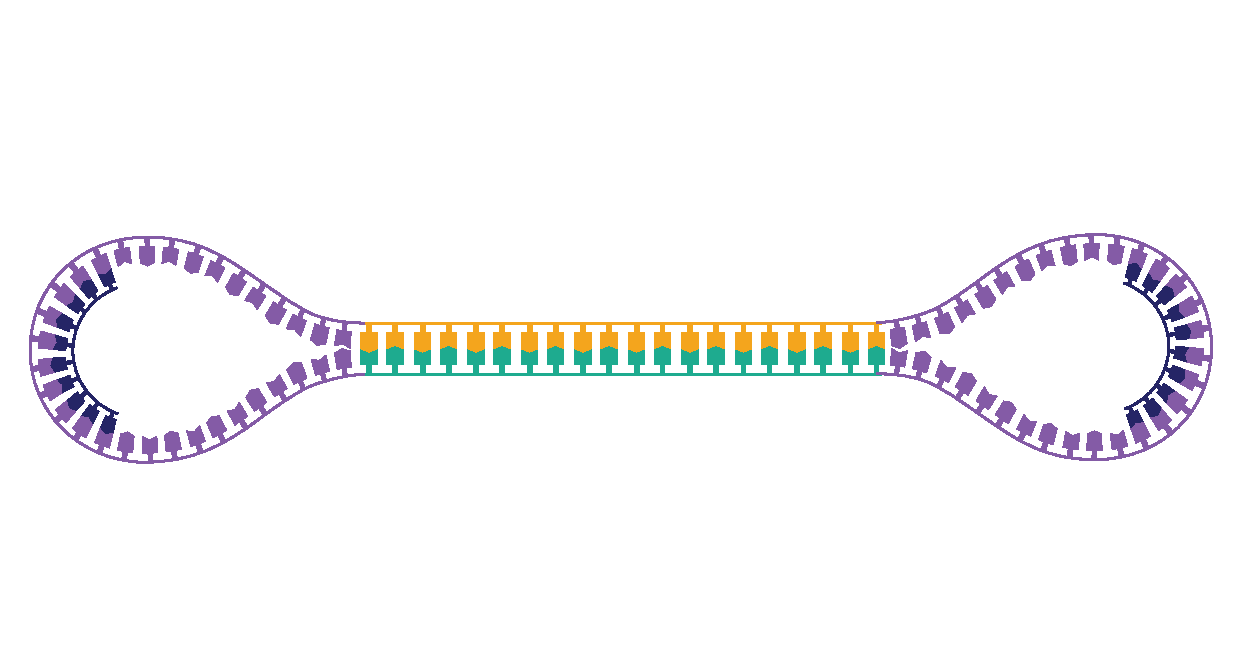
\includegraphics[width=\textwidth]{Vector/SMRTbell_template.pdf}
\end{centering}
\floatfoot{A hairpin adapter in purple is attached to a double-stranded DNA. The forward strand is coloured in yellow and reverse strand is coloured in green. The primer that DNAP binds to is coloured in black.}
\end{figure}

The loading of SMRTbell template into a ZMW follows a Poisson distribution, and typically 30-50\% of the ZMWs are classified as productive ZMWs, where a single DNAP successfully initiates and completes rolling circle sequencing. SMRT sequencing initially used $\Phi$29 DNAP due to its high processivity, minimal amplification bias and ability to perform strand displacement DNA synthesis \cite{Eid2009-ol}. Additionally, $\Phi$29 DNAP was engineered through site-directed mutagenesis to enable the incorporation of fluorophore-labelled deoxyribonucleoside triphosphate (dNTP) during DNA elongation \cite{Eid2009-ol, Korlach2008-fv}. 

After the successful loading of the SMRTbell template, free nucleotides are released above the ZMW array, and they diffuse in and out of the ZMW. DNAP binds to the template and incorporates the correct nucleotide into the growing DNA strand. Upon nucleotide incorporation, DNAP cleaves the fluorophore from the nucleotide, resulting in the synthesis of native DNA molecules. DNAP continues DNA elongation until DNA replication is terminated.

The length of the DNA synthesis is dependent on DNAP processivity and the presence of bulky DNA damage on the template DNA, which can cause premature termination of replication. Illumination from the laser below the glass surface excites the fluorophore, and the emitted fluorescence is measured. An image processor leverages the temporal difference between the diffusion of free nucleotides (which occurs in microseconds) and nucleotide incorporation (which occurs in milliseconds) to distinguish the background fluorescence from free nucleotides and fluorescence from nucleotide bound to DNAP. Critically, the size and shape of the ZMW prevents laser light from passing through the ZMW, confining the illumination to the bottom of the ZMW and improving the signal-to-noise ratio. As the four dNTPs are each labelled with a different fluorophore, each nucleotide can be identified from their unique fluorescence \cite{Eid2009-ol}. 

DNAP kinetics can also be used to detect DNA base modifications. DNAP kinetics is is comprised of duration of fluorescence pulse, known as pulse width, and the duration between successive fluorescence pulses, referred to as interpulse duration (IPD) \cite{Flusberg2010-ub}. To date, DNAP kinetics has been used to detect including base modifications such as N6-methyladenine, 5-methylcytosine (5mC) and 5-hydroxymethylcytosine \cite{Flusberg2010-ub} and DNA damage such as O6-mmethylguanine, 1-methyladenine, O4-methylthymien, 5-hydroxycyostine, 5hydroxyuracil, 5-hydroxymethyluyracil and thymine dimers \cite{Clark2011-jz}. 

PacBio sequencing instrument initially generated continuous long read (CLR) with 10-15\% error rate \cite{Eid2009-ol}. This was due to an inherent trade-off between read length and read accuracy while maintaining DNAP processivity as a constant. The earlier generations of DNAP had insufficient processivity to sequence both the forward and reverse strands of a SMRTbell template multiple times (Figure \ref{figure:clr-sequencing}).

\begin{figure}[h!]
\caption{CLR sequencing}
\label{figure:clr-sequencing}
\begin{centering}
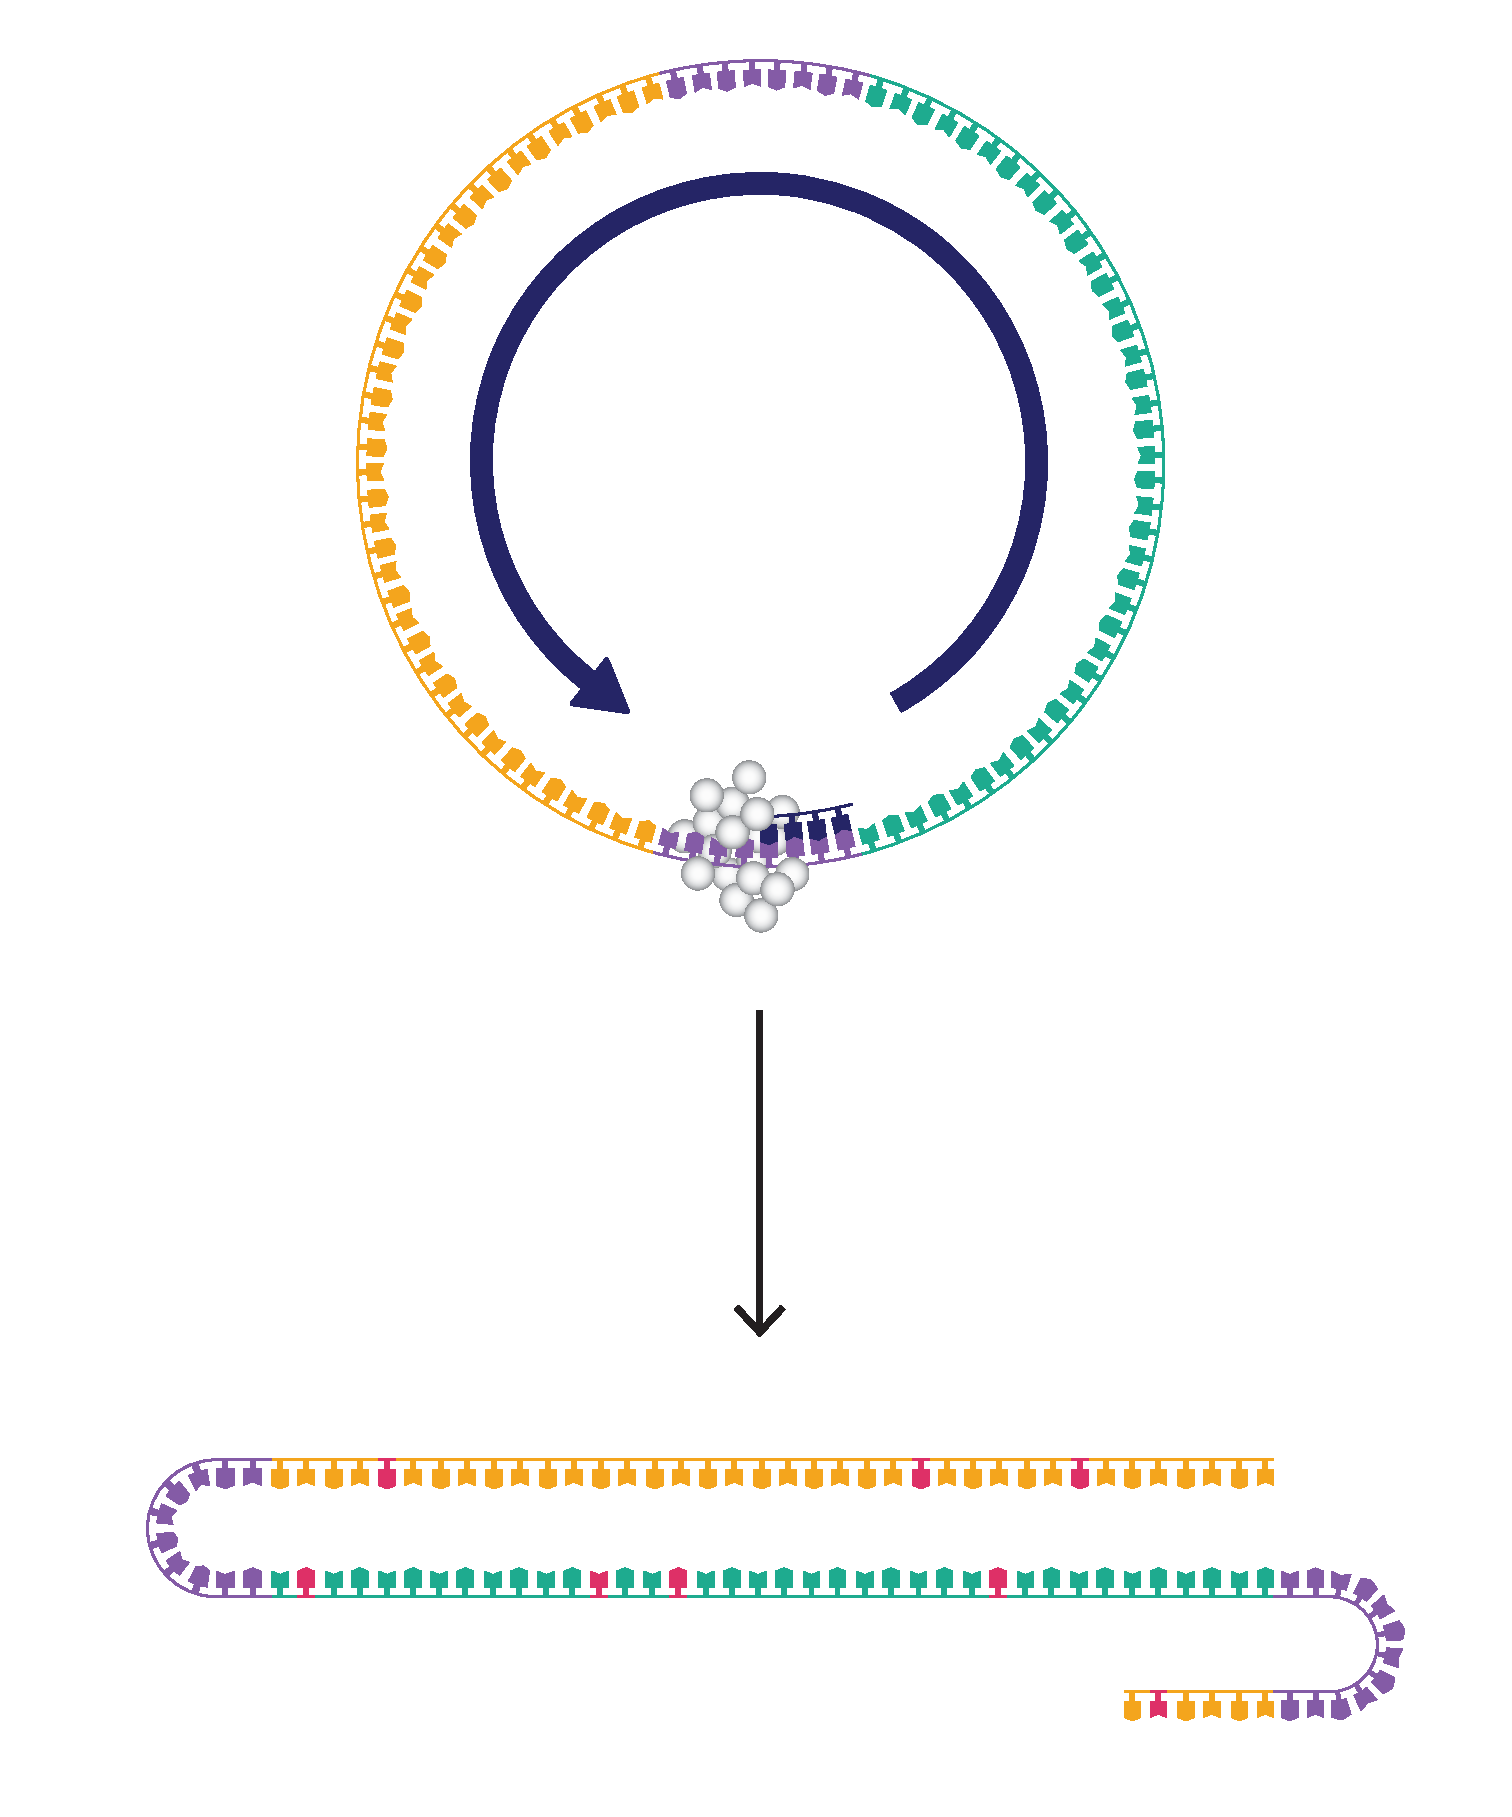
\includegraphics[width=0.8\textwidth]{Vector/CLR_sequencing.pdf}
\end{centering}
\floatfoot{DNAP used in CLR sequencing didn't have sufficient processivity to enable multiple-pass sequencing of read-of-insert greater than 10kb. Here, DNAP sequences the forward and reverse strand once.}
\end{figure}

In contrast, the more recent generations of DNAP possess sufficient processivity to sequence both the forward and reverse strand of long SMRTbell templates (>10kb) multiple times, resulting tin the generation of long and accurate reads \cite{Wenger2019-pw}. Circular consensus sequence (CCS) reads from the Sequel II instrument are reported to have an error rate of 0.1-1\% \cite{Wenger2019-pw} (Figure \ref{figure:ccs-sequencing}).

\begin{figure}[htbp!]
\caption{CCS sequencing}
\label{figure:ccs-sequencing}
\begin{centering}
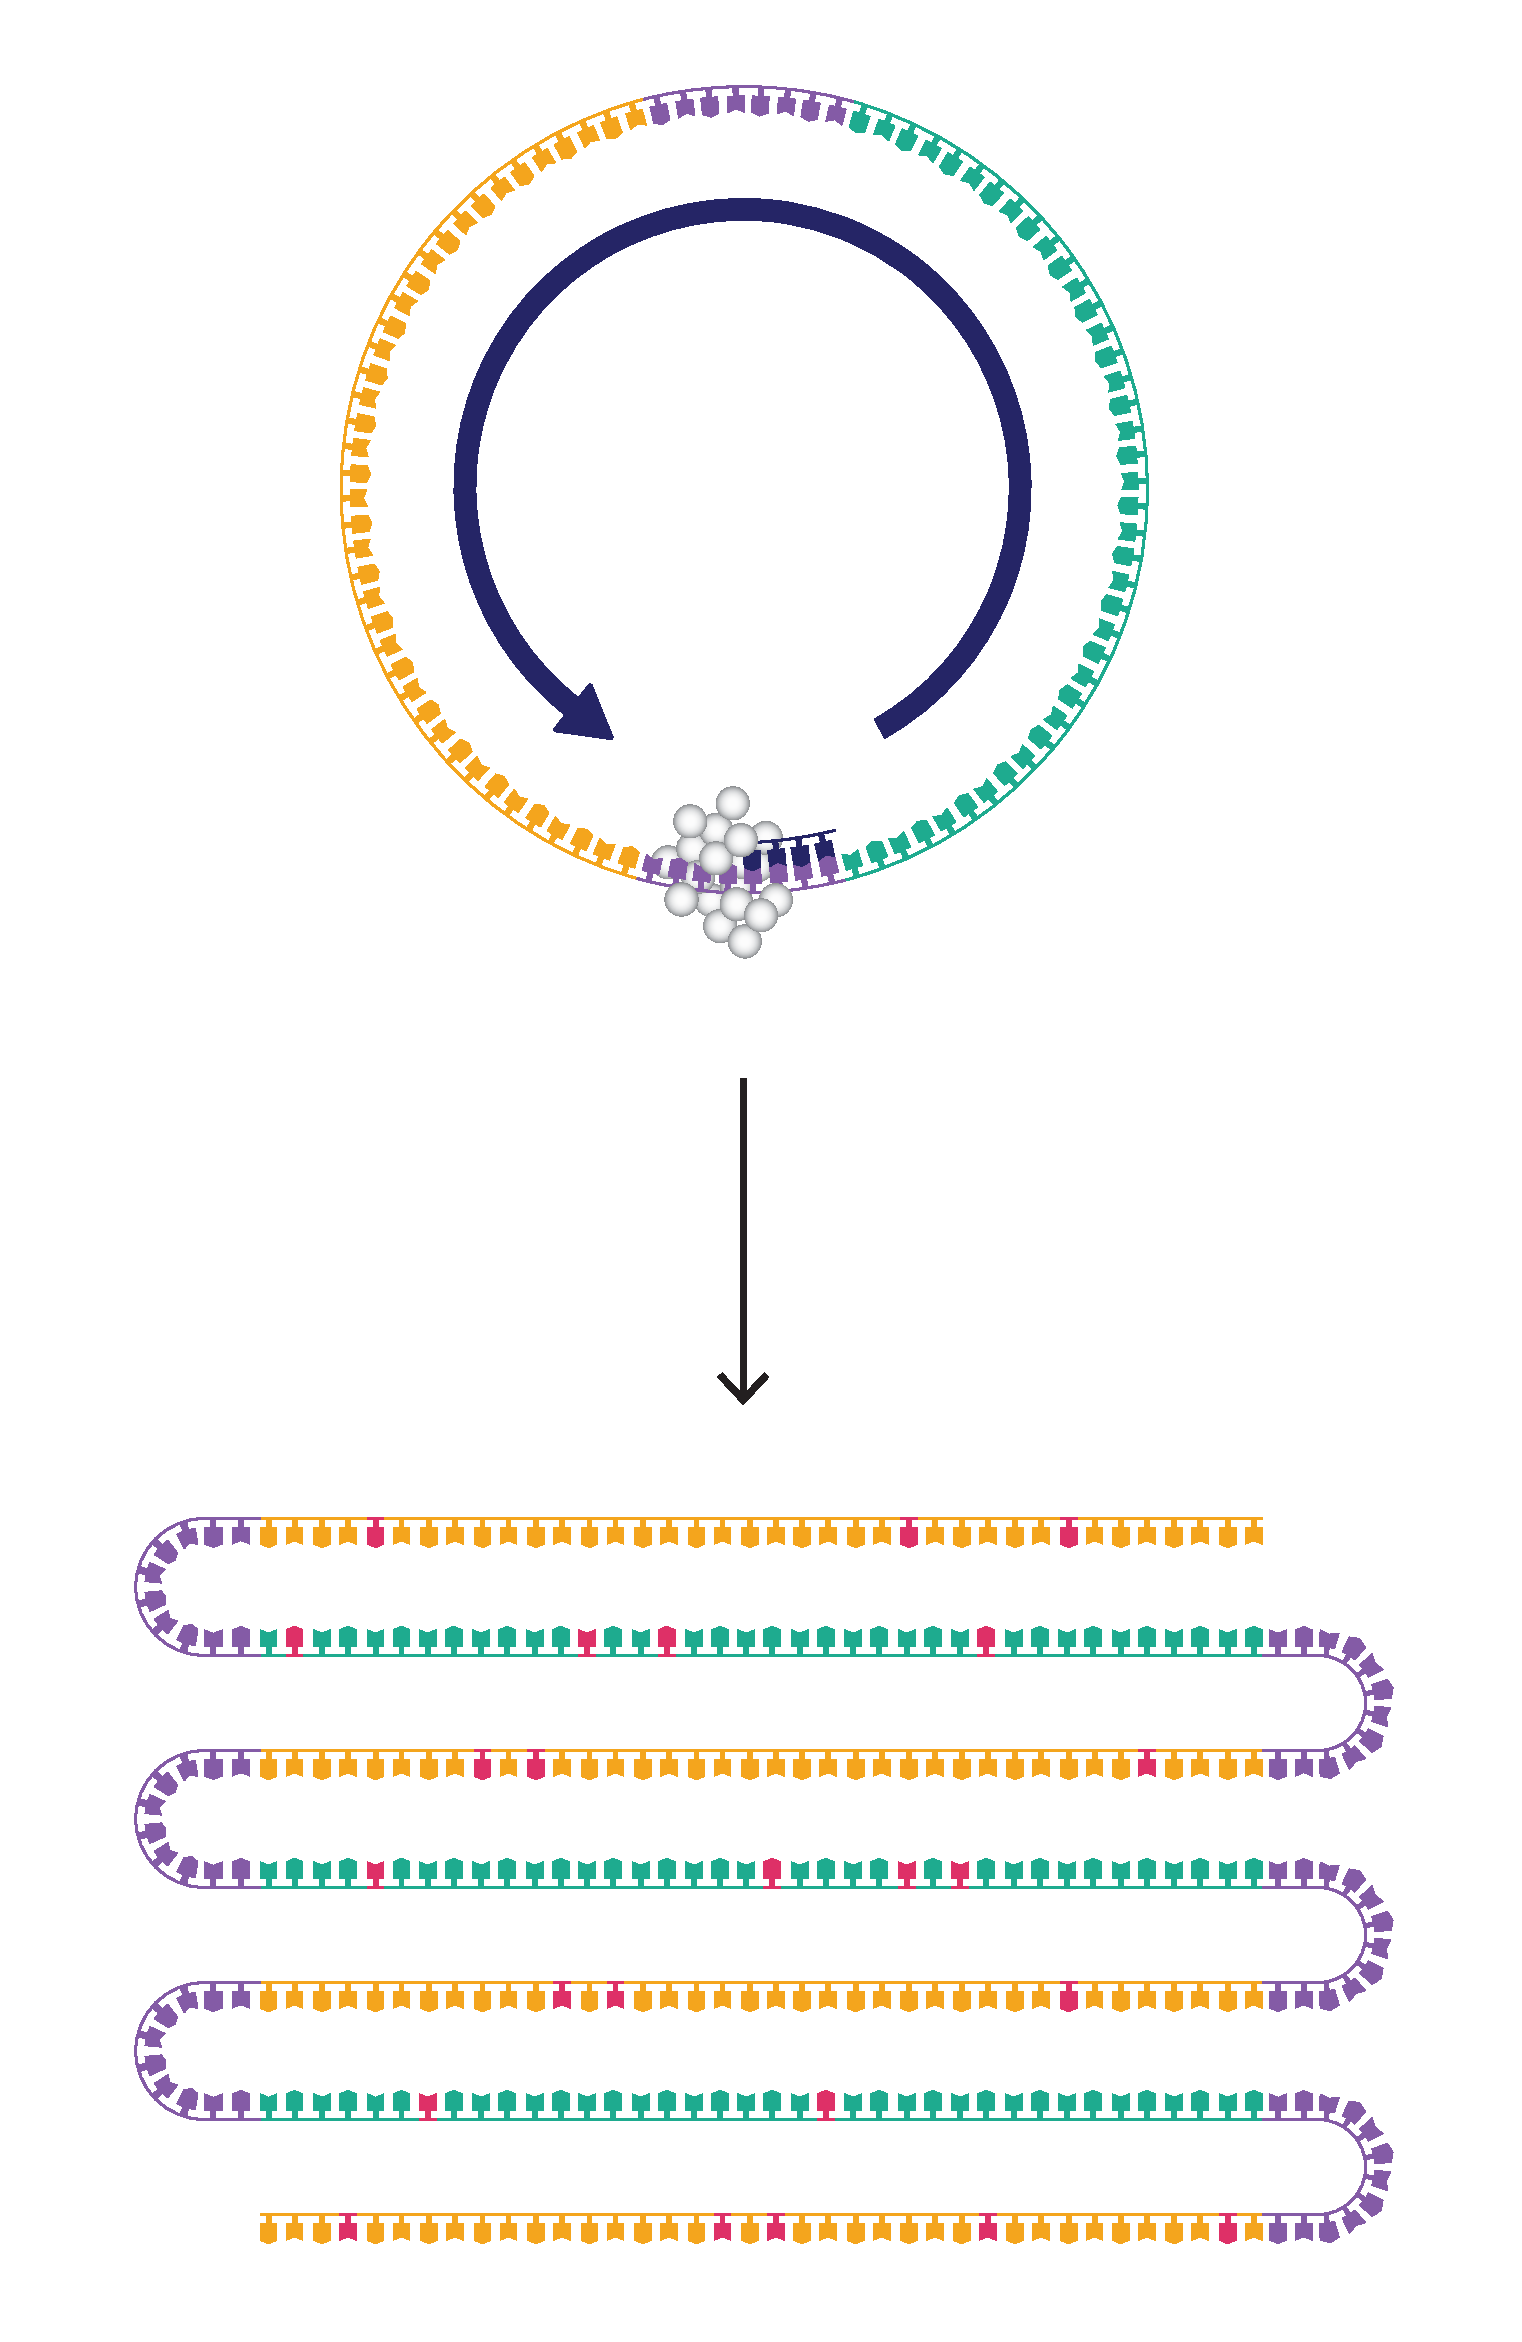
\includegraphics[width=0.8\textwidth]{Vector/CCS_sequencing.pdf}
\end{centering}
\floatfoot{In contrast, DNAP used in CCS sequencing have sufficient processivity to sequence a 20kb read-of-insert 10 to 16 times.}
\end{figure}

The PacBio RS instrument, equipped with the first generation of polymerase and chemistry (P1-C1), produced CLR reads with an average length of 1,500 bp with an error rate of 10-15\% \cite{Quail2012-cx}. In addition, the first generation of SMRTcells had 150, 000 ZMWs \cite{Rhoads2015-pk}. In contrast, the latest PacBio Revio instrument generates CCS reads with an average read length of around 20,000 bp with an error rate of 0.1-1\% \cite{revio2022}. Moreover, the SMRTcell for the PacBio Revio instrument has 25 million ZMWs. Therefore, the sequence throughput of SMRTcells has increased exponentially, from approximately 112 million CLR bases per SMRTcell to 250 billion CCS bases per SMRTcell, assuming that approximately half of the ZMWs are productive ZMWs. As a result, a single SMRTcell can generate 30-fold CCS sequence coverage of a human genome under one thousand dollars. The resulting output not only facilitates \textit{de novo} assembly \cite{Nurk2020-gu, Cheng2021-ij} but also enables haplotype phasing of \cite{Patterson2015-an} and detection of both germline mutations \cite{Poplin2018-ub} and base modifications \cite{Tse2021-or}. 


\subsection{Long-read sequencing applications}

The high error rate of CLR reads, coupled with lower sequence throughput compared to Illumina sequencing instruments, initially limited the applications of CLR reads to microbial genome assembly \cite{Chin2013-hp}, targeted BAC clone sequencing to close gaps in the human reference genome \cite{Huddleston2014-rs}, nucleotide-resolution structural variation detection for rare genetic disease diagnostics \cite{Loomis2013-ca}, and the study of hidden genetic variations \cite{Chaisson2015-zz}. The introduction of the P6-C4 chemistry and PacBio RSII instrument marked a significant milestone, leading to a substantial increase in CLR read length and sequence throughput \cite{Rhoads2015-pk}. This breakthrough enabled the successful assembly of larger and more repetitive mammalian genomes, including those of great apes such as gorillas \cite{Gordon2016-ho}, chimpanzees \cite{Kronenberg2018-wy}, and orangutans \cite{Kronenberg2018-wy}. Furthermore, CCS sequencing represents another significant advancement that enables us to explore previously unexplored biological phenomena.

\subsubsection{Genome assembly}

Genome assembly aims to determine the entire the genetic information of an organism. It can be divided into four distinct stages: 1) shotgun or hierarchical shotgun sequencing and quality control, 2) all-to-all read alignments to find overlaps between reads and the generation of contigs from overlapping reads 3) the use of long-range information to order and orient contigs into scaffolds, and 4) finishing the genome through polishing and gap closing.

The contiguity and completeness of the assembly depend on the repeat content and sequence coverage of the genome \cite{Lander1988-hu}. When a read originates from a repetitive sequence, it may overlap with another read containing a similar or identical repeat sequence, resulting in a false overlap in the assembly graph. If a read longer than the repeat length is not present, repeat-induced overlap can lead to either gaps or collapsed regions in the genome assembly.

To minimise the number of potential assembly errors, the Human Genome Project (HGP) adopted hierarchical shotgun sequencing of 100-200 kb bacterial artificial chromosome (BAC) clones to construct the human reference genome \cite{Lander2001-du}. The use of BAC clones simplifies the genome assembly process by reducing the complexity of the problem to a local assembly challenge.

In contrast, shotgun sequencing based \textit{de novo} assembly requires read length to be longer than the repeat length to assemble high-quality reference genomes. Read length must be longer than the repeat length to ensure that unique sequences not found elsewhere in the genome flank the repetitive sequence in the read. This enables the unique placement of a read in an assembly graph. In contrast to short reads, long reads from the SMRT platform can span the most commonly occurring repeats such as $\sim$300 bp short interspersed nuclear element (SINE) and $\sim$5000 bp long interspersed nuclear element (LINE). Hence, long reads can be unambiguously aligned to the reference genome and can be used to resolve repeat-induced false overlaps in the assembly graph. 

A new generation of assembly algorithms based on de Brujin graph \cite{Lin2016-vl}, string graph \cite{Myers2005-ei, Chin2016-at} and overlap layout consensus (OLC) \cite{Koren2017-cq} were developed to leverage these long reads and enable end-to-end assembly of microbial genomes\cite{Chin2013-hp, Bashir2012-cs} and large mammalian genomes \cite{Chin2016-at, Koren2017-cq}. \textit{De novo} assembly algorithms perform all-against-all pairwise read alignments to identify overlaps between pairs of reads and the reliable overlaps are connected to produce contigs. The length of the overlap and the shared sequence identity between the overlap determines the reliability of the overlap. A repeat-induced overlap is generated when a read, derived from a repeat sequence, aligns to another read with a similar repeat sequence. If these repeat-induced false overlaps are left unresolved, fragmented contigs are generated from the assembly graph. 

As long reads often have unique sequences flanking the repeat sequence, repeat-induced overlaps that could not be resolved with short reads can be easily unentangled with long reads, often enabling the generation of chromosome-arm level contigs \cite{Nurk2020-gu, Cheng2021-ij}. CCS reads, with their higher base accuracy, excel at distinguishing more recently diverged repeats \cite{Nurk2022-dv}. Long reads can also unravel divergences in the assembly graph, often referred to as a bubble, resulting from structural differences between the two haplotypes and produce haplotype phased contigs (haplotigs) \cite{Chin2016-at}. As a result, the contigs produced from long reads have unparalleled completeness and contiguity compared to that produced from short reads \cite{Gordon2016-ho}, reigniting interest for the development of \textit{de novo} assembly and scaffolding algorithms.  

To complement the contigs produced from long reads, several new sequencing, physical mapping, and assembly and scaffolding algorithms have been developed. For instance, haplotype-resolved assemblies can be generated by leveraging the parent-specific kmers available through trio-sequencing \cite{Koren2018-wg} or through haplotype phasing using Strand-sequencing \cite{Porubsky2021-ct}.  Genome maps from Bionano Genomics have also been used to correct misassemblies, and to order and orient contigs into chromosome-arm level scaffolds \cite{Pendleton2015-ue}. Above all, chromosome-length scaffold construction has become routine through Hi-C scaffolding and the ability to visualise \cite{Robinson2018-os} and manually inspect Hi-C contact matrix for assembly curation\cite{Dudchenko2018-yl}. The ultra-long read (>100kb) library preparation and sequencing using the ONT platform \cite{Jain2018-zh} also facilitates the full-length sequencing of individual BAC clones \cite{Jain2018-mg} and closing of gaps in the genome that could not be assembled with CCS reads. The completion of the gapless T2T-CHM13 genome, including the short arms of five acrocentric chromosomes and centromeric satellite array, represents the latest advances in sequencing and assembly algorithms \cite{Nurk2022-dv}. 

\subsubsection{Germline and somatic mutation detection}

To date, long reads have been successfully used for germline SNP and indel \cite{Poplin2018-ub}, as well as for structural variation detection \cite{Chaisson2015-zz}. However, The lower base accuracy and higher per-base sequencing cost have limited the use of CLR reads for SNP and indel detection. Until the introduction of CCS reads, the primary advantage of CLR reads has been their ability to access regions of the genome that were previously inaccessible with short reads, especially for for nucleotide-resolution structural variation detection. 

Short-read based structural variation detection reads relies on changes in sequence coverage for copy number variation (CNV) detection \cite{Abyzov2011-xl} and identification of discordant read pairs with aberrant distance and orientation for breakpoint, translocation and inversion detection \cite{Alkan2011-dv}. In contrast, long reads enable nucleotide-resolution structural variation detection through direct comparison of the read to the reference genome. Long-read based structural variation detection is particularly more sensitive towards short tandem repeat (STR), SINE and LINE insertion detection \cite{Chaisson2015-zz, Sedlazeck2018-oh, Denti2022-ux}. If the length and base accuracy of the long read is not sufficient to detect structural variations at the required resolution, \textit{de novo} assembled contigs facilitate the identification of larger and more complex structural rearrangements \cite{Nattestad2016-og}.

CHM1 CLR reads, for example, were used to identify approximately 26,000 structural variations that were recalcitrant to detection using short reads \cite{Chaisson2015-zz}. The number of structural variations detected with long reads is at least double that detected with short reads. Although the number of structural variations is orders of magnitude smaller than the number of SNPs and indels, they can alter a greater number of bases and have a more pronounced impact on an individual's phenotype \cite{Weischenfeldt2013-tl}. Additionally, structural variations can induce conformational changes in the three-dimensional configuration of the genome \cite{Spielmann2018-fm}.

The diagnosis rate of rare genetic diseases is estimated to be approximately 30-40\% with short read sequencing \cite{Wright2023-et}, which is not surprising considering the difficulty of their detection. In contrast, long read sequencing has repeatedly demonstrated its superiority for identification of pathogenic mutations. For instance, repeat expansions and accompanied hypermethylation are common causes of neurological diseases \cite{Zhou2022-ci}, and SMRT sequencing enables their simultaneous detection \cite{Loomis2013-ca}. Moreover, STR expansion detection in patients with spinocerebellar ataxia type 10 (SCA10) with long reads has demonstrated that both the repeat sequence and the size of the repeat expansion is associated with the severity of the disease \cite{McFarland2015-qh}. The ability to detect haplotype phased germline and epigenetic modifications has renewed interest to explore hidden genetic variation and to accelerate the identification of pathogenic mutations in patents with rare genetic diseases \cite{Miller2021-lt}. For instance, the human genome structural variation consortium is re-sequencing some of the samples from the 1000 genomes project with the SMRT platform to develop new structural variation detection algorithms and to study the genomic architecture \cite{Ebert2021-zk}. 

Although long-read sequencing technologies offer numerous advantages compared to short-read sequencing technologies for somatic structural rearrangement detection, long reads have been underutilised in somatic mutation detection. Only a handful of samples have been sequenced to interrogate somatic structural rearrangements using long reads \cite{Nattestad2018-tr, Sakamoto2020-nq, Fujimoto2021-kc}. Moreover, somatic substitution and indel detection algorithms, to our knowledge, have not been developed to leverage CLR or CCS reads. Hence, I believe that a series of method development is required to enable the adoption of long-read sequencing for cancer genomics research. 

\section{Tree of Life}

The Tree of Life is a recurring cultural and religious symbol that represents enlightenment, eternal life, and the universe. Charles Darwin first used the Tree of Life to illustrate the implications of natural selection and speciation (Figure \ref{figure:tree-of-life}) \cite{Darwin1859}. In particular, Darwin used the Tree of Life as a symbolic metaphor to represent the emergence and extinction of new species, as well as the interconnectedness of different species through a shared ancestor.


\begin{figure}[htbp!]
\caption{Tree of Life}
\label{figure:tree-of-life}
\begin{centering}
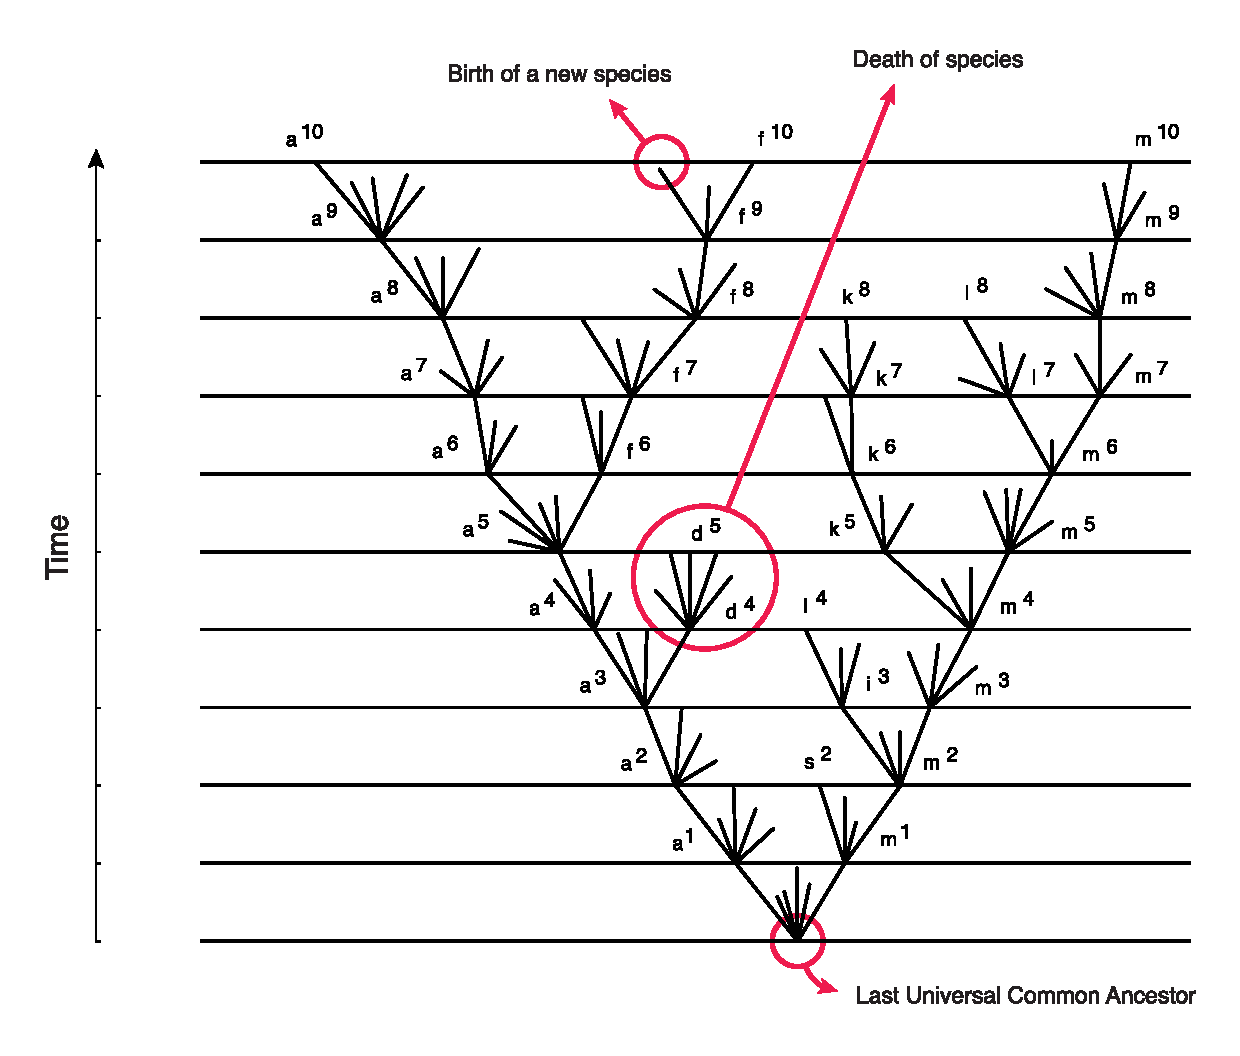
\includegraphics[width=\textwidth]{Vector/tree_of_life.pdf}
\end{centering}
\floatfoot{A reproduction of the Tree of Life from Darwin’s \textit{On the Origin of Species} with personal annotations in red}
\end{figure}

At the very root of the Tree of Life lies the last universal common ancestor (LUCA), from which all living organisms are believed to have descended. Each branching point depicts the emergence of a new group of species as a consequence of the struggle for existence. Each leaf, the endpoints of the branches, embodies distinct species and is the product of billions of years of evolution. 

Since the publication of Darwin's seminal work, \textit{On the Origin of Species} \cite{Darwin1859}, significant scientific advancements have been made. Nucleic acid has been determined to be the universal carrier of genetic information \cite{Avery1944-lr}, the double helix structure of the DNA has been discovered \cite{Watson1953-lr}, and it has been established that the same genetic code is used universally to encode amino acids across all forms of life \cite{Woese1968-lr}. These remarkable discoveries provide strong evidence supporting Darwin's conjecture that all living species on Earth share a common ancestor.

The prohibitive cost of clone-by-clone sequencing for reference genome construction, the inability to produce high-quality reference genomes from short-read sequencing and the challenges of somatic mutation detection in normal tissues have prevented the detection and analysis of somatic mutations, the source of raw materials for natural selection, in other species.

\subsection{Peto’s paradox}

The study of somatic mutations and mutational processes in other species is a captivating area of research that sheds light on the underlying mechanisms of aging and the occurrence of cancer. Sir Richard Peto observed that there is no clear correlation between the number of cells and the incidence of cancer in other animals \cite{Peto2016-wf, Vincze2022-tw}. Because somatic mutational processes alter the genome of individual cells, and the number of somatic mutations increases with age, it might be expected that larger animals with a greater number of cells and long-lived species would have an elevated risk of developing cancer. However, elephants provide an interesting counter example. Elephants have over one hundred times the number of cells compared to humans, but they have a cancer mortality rate of 4.81\%, in contrast to the 11-25\% cancer mortality rate observed in humans \cite{Abegglen2015-ao}. The analysis of the elephant genome has revealed that the elephant genome possesses 20 copies of the TP53 gene, whereas the human genome contains 2 copies of the TP53 gene \cite{Sulak2016-ld}, which is a tumour suppressor gene that is critical for maintaining genome stability \cite{Vousden2009-wd}. The higher number of TP53 genes in the elephant genome is believed to be one of the primary reasons why elephants have a lower incidence of cancer.

\subsection{Somatic mutation theory of ageing}

The somatic mutation theory of ageing suggests that the gradual accumulation of somatic mutations leads to a decline in cellular function, ultimately contributing to the ageing process \cite{Szilard1959-ru}. This theory also implies that shorter-lived species will have a higher somatic mutation rate than longer-lived species. A recent study of somatic mutation rate in colonuc crypt across various mammalian species of different ages and lifespan have confirmed that the somatic mutation rate is inversely proportional to the lifespan of the mammalian species \cite{Cagan2022-yn}. Thus, longer-lived species tend to have a lower somatic mutation rate. It is unclear whether this relationship between somatic mutation rate and the species’ lifespan holds true in other order, phyla, and kingdom.

\subsection{Darwin Tree of Life project}

The advancements in single-molecule sequencing technologies, accompanied by the concurrent development of new generations of \textit{de novo} assembly and scaffolding algorithms, and the ability to produce high-quality chromosome-length scaffolds at a fraction of the cost of hierarchical shotgun sequencing have brought new enthusiasm to assemble high-quality reference genomes for vertebrates \cite{Rhie2021-dq} and all eukaryotic diversity on Earth \cite{Lewin2018-zf}. 

The Darwin Tree of Life (DToL) project is an ambitious project that aspires to build reference genomes for all 70, 000 eukaryotic species in Britain and Ireland \cite{Darwin_Tree_of_Life_Project_Consortium2022-ma}. At the time of writing, the DToL project has sequenced approximately 800 species, completed the assemblies of approximately 600 species, and raw data and reference genomes have been made available to the public.

I hypothesised that the availability of CCS reads and reference genomes through the DToL project presents a unique opportunity to discover new somatic mutational processes across the Tree of Life. 

\section{Thesis objectives}

I have organised the remainder of this PhD thesis as follows. In chapter 2, I measure the CCS error rate and assess the potential for somatic mutation using CCS reads. I also introduce himut, a method that enables the detection of somatic mutations, agnostic of clonality and species. In chapter 3, I use himut to detect somatic mutations from eukaryotic species in the DToL project, describe the newly identified mutational signatures and measure the contribution of these mutational signatures to both germline and somatic mutations observed in each species.


